\documentclass[../../main.tex]{subfiles}

\begin{document}

\begin{figure}[!tbp]
    \centering
    \begin{subfigure}[b]{0.4\textwidth}
    \centering
    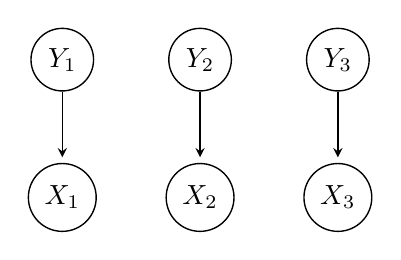
\begin{tikzpicture} [-> , >= stealth, shorten >= 2 pt, line width = 0.5pt, node distance = 1.75cm]
        \node [draw, circle] (y1) {$Y_1$};
        \node [draw, circle] (y2) [right of = y1] {$Y_2$};
        \node [draw, circle] (y3) [right of = y2] {$Y_3$};
        
        \node [draw, circle] (x1) [below of = y1] {$X_1$};
        \node [draw, circle] (x2) [below of = y2] {$X_2$};
        \node [draw, circle] (x3) [below of = y3] {$X_3$};
        
        \path (y1) edge (x1);
        \path (y2) edge (x2);
        \path (y3) edge (x3);
        
    \end{tikzpicture}
    \caption{A Na{\"i}ve Bayes classifier applied to the part-of-speech tagging problem.}
  \end{subfigure}
  \hfill
  \begin{subfigure}[b]{0.4\textwidth}
    \centering
    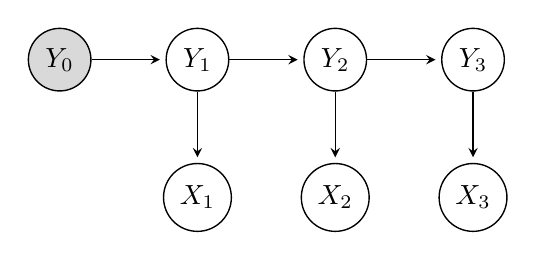
\begin{tikzpicture} [-> , >= stealth, shorten >= 2 pt, line width = 0.5pt, node distance = 1.75cm]
        \node [draw, circle, fill=gray!30!white] (start) {$Y_0$};
        \node [draw, circle] (y1) [right of = start] {$Y_1$};
        \node [draw, circle] (y2) [right of = y1] {$Y_2$};
        \node [draw, circle] (y3) [right of = y2] {$Y_3$};
        
        \path (start) edge (y1);
        \path (y1) edge (y2);
        \path (y2) edge (y3);
        
        \node [draw, circle] (x1) [below of = y1] {$X_1$};
        \node [draw, circle] (x2) [below of = y2] {$X_2$};
        \node [draw, circle] (x3) [below of = y3] {$X_3$};
        
        \path (y1) edge (x1);
        \path (y2) edge (x2);
        \path (y3) edge (x3);
        
    \end{tikzpicture}
    \caption{A hidden Markov model applied to the part-of-speech tagging problem.}
\end{subfigure}
\caption{My flowers.}
\end{figure}

\end{document}